\documentclass[11pt,a4paper]{article}
\usepackage[utf8]{inputenc}
\usepackage[english]{babel}
\usepackage{amsmath}
\usepackage{amsfonts}
\usepackage{amssymb}
\usepackage[left=2.5cm,right=2.5cm,top=2cm,bottom=2cm]{geometry}
\usepackage[onehalfspacing]{setspace}
\usepackage{booktabs}
\usepackage{graphicx}
\usepackage{xcolor}
\definecolor{DueMain}{RGB}{0,76,147}

\usepackage{hyperref}
\hypersetup{
    colorlinks = true,
    linkcolor = {DueMain},
    citecolor = {DueMain},
    urlcolor = {DueMain}
    }
\usepackage{subcaption}
\usepackage{eurosym}
\usepackage{array}
\newcommand{\specialcell}[2][l]{%
  \begin{tabular}[#1]{@{}l@{}}#2\end{tabular}}
  \newcommand{\specialcellc}[2][c]{%
  \begin{tabular}[#1]{@{}c@{}}#2\end{tabular}}
\newcolumntype{L}[1]{>{\raggedright\arraybackslash}p{#1}} % linksbündig mit Breitenangabe

\usepackage[autostyle]{csquotes}
\usepackage[style=authoryear-icomp, uniquelist=false, maxnames=5, maxcitenames=2, minnames=1, natbib=true, isbn=false, doi=true, url=true, date=year, giveninits=true, backend=biber]{biblatex}

\DeclareFieldFormat[article]{volume}{\mkbibbold{#1}}
\DeclareFieldFormat{pages}{#1}
\renewcommand{\labelnamepunct}{\addspace}

\renewbibmacro{in:}{%
  \ifentrytype{article}{}{\printtext{\bibstring{in}\intitlepunct}}}
\renewbibmacro*{name:andothers}{% Based on name:andothers from biblatex.def
  \ifboolexpr{
    test {\ifnumequal{\value{listcount}}{\value{liststop}}}
    and
    test \ifmorenames
  }
    {\ifnumgreater{\value{liststop}}{1}
       {\finalandcomma}
       {}%
     \andothersdelim\bibstring[\emph]{andothers}}
    {}}

\addbibresource{SupplementaryMaerial.bib}
\DeclareDelimFormat[cbx@textcite]{nameyeardelim}{\addspace}
\setcounter{biburlnumpenalty}{100}
\citetrackerfalse
\usepackage{authblk}
\usepackage[normalem]{ulem}
\usepackage{microtype}
\begin{document}
\date{\ }
\title{\textbf{Is the Eurozone disintegrating?}\\  \textbf{Macroeconomic divergence, structural polarization, trade and fragility}\thanks{Supported by funds of the Oesterreichische Nationalbank (Austrian Central Bank, Anniversary Fund, project number: 17383). CG acknowledges funding by the Austrian Science Fund (FWF) under grant number ZK 60-G27. You can contact the authors via Email: \href{mailto:claudius@claudius-graebner.com}{claudius@claudius-graebner.com} (CG), \href{mailto:heimberger@wiiw.ac.at}{heimberger@wiiw.ac.at} (PH), \href{mailto:jakob.kapeller@uni-due.de}{jakob.kapeller@uni-due.de} (JK) and \href{mailto:bernhard.schuetz@jku.at}{bernhard.schuetz@jku.at} (BS).} \\
Supplementary material}

\author[a,b,c]{Claudius Gr\"abner}
\author[a,d]{Philipp Heimberger}
\author[a,b]{Jakob Kapeller}
\author[a,e]{Bernhard Sch\"utz}
% Affiliations (Buchstaben muessen zu den Zeilen davor korrespondieren)
\affil[a]{Institute for Comprehensive Analysis of the Economy (ICAE), Johannes Kepler University, Linz, Aubrunnerweg 3a, 4040 Linz, Austria.}
\affil[b]{Institute for Socio-Economics, University of Duisburg-Essen, Lotharstr. 65, 47057 Duisburg, Germany.}
\affil[c]{ZOE. Institute for Future-Fit Economies, Thomas-Mann-Str. 36, 53111 Bonn, Germany.}
\affil[d]{The Vienna Institute for International Economic Studies, Rahlgasse 3, 1060 Vienna, Austria}
\affil[e]{Department of Economics, Altenbergerstraße 69, Johannes Kepler University, Linz , Austria}

\setcounter{Maxaffil}{0}
\renewcommand\Affilfont{\itshape\small}


\maketitle
\begin{abstract}
The supplementary material describes our data sources (section \ref{ap:data})
and discusses the index of economic complexity (section \ref{ap:eci}).
It also contains a robustness check of our results on the polarization in terms of export baskets and explicates the derivation of the deviation of actual exports from expected exports plotted in figure 8 of the main paper (section \ref{ap:robust}). 
Finally, it supplies the complexity distribution plots for the export baskets of all Eurozone countries (section \ref{ap:exp-densities}).

The data set and the code to reproduce all empirical analyses of the paper and the appendix are available on Github: \href{https://github.com/graebnerc/disintegrating-europe}{https://github.com/graebnerc/disintegrating-europe}. An accompanying data publication also exists \citep{Grabner:2019data}

\end{abstract}

\newpage

\appendix
\section{Data sources}
\label{ap:data}
The data we used were compiled from the following sources:

\begin{center}
\begin{tabular}{ c c }
\toprule
\textbf{Variable} & \textbf{Source} \\ 
\midrule 
Long-term interest rate & OECD (May 2017) \\
Unemployment rate & AMECO (Spring 2017)\\
GDP growth & AMECO (Spring 2017)\\
Current account to GDP & AMECO (Spring 2017)\\
Population & United Nations Population Division\\
Household debt & OECD (May 2017)\\
Corporate debt & OECD (May 2017)\\
Government debt & AMECO (Spring 2017)\\
Trade balances & IMF Direction of Trade (July 2017)\\
Export data & \citet{AtlasData}, accessed in May 2019\\
\bottomrule
\end{tabular} 
\end{center}

For the descriptive statistics see table \ref{tab:desc-stats}.

\begin{table}[!htbp] 
\centering 
\begin{tabular}{@{\extracolsep{5pt}}lccccc} 
\toprule 
\textbf{Statistic} & \multicolumn{1}{c}{\textbf{N}} & \multicolumn{1}{c}{\textbf{Mean}} & \multicolumn{1}{c}{\textbf{St. Dev.}} & \multicolumn{1}{c}{\textbf{Min}} & \multicolumn{1}{c}{\textbf{Max}} \\ 
\hline \\[-1.8ex] 
Current\_account\_balance\_to\_GDP & 216 & 0.563 & 5.816 & $-$15.849 & 12.537 \\ 
GDP\_growth & 216 & 1.767 & 3.380 & $-$9.133 & 26.276 \\ 
Public\_debt\_to\_GDP & 216 & 73.851 & 35.584 & 6.456 & 179.732 \\ 
Unemployment\_rate & 216 & 8.762 & 4.685 & 1.900 & 27.500 \\ 
complexity\_HH & 183 & 1.284 & 0.527 & 0.120 & 2.255 \\ 
debt\_corp\_nf\_percGDP & 205 & 151.399 & 73.626 & 41.474 & 444.299 \\ 
debt\_gen\_gov\_percGDP & 207 & 83.456 & 36.124 & 12.643 & 185.237 \\ 
debt\_hh\_npish\_percGDI & 188 & 113.280 & 53.950 & 21.860 & 268.397 \\  
interest\_lt & 213 & 4.052 & 2.340 & $-$0.177 & 22.497 \\ 
population & 204 & 26,094.900 & 26,508.460 & 431.264 & 81,965.830 \\ 
\bottomrule
\end{tabular} 
\caption{The descriptive statistics for the data used. Except \texttt{complexity\_HH} and \texttt{population} all are reported in per cent.}  \label{tab:desc-stats} 
\end{table}

\newpage

\section{The economic complexity index}
\label{ap:eci}
The index of economic complexity (ECI) was first introduced in \citet{Hidalgo:2007cp} and further explicated in \citet{Hidalgo:2009be} and \citet{Hausmann:2013vj}.
For the underlying theory and a further interpretation, according to which the fundamental driving force for the development of nations is their ability to accumulate more and more information, see \citet{Hidalgo:2015vs}.

The index can be understood as a measure of the knowledge intensity of an economy, or, in other words, the amount of technological capabilities present in this economy. 
Its prominence stems from the fact that it is a good predictor for future growth rates of national economies, indicating that ``countries tend to approach the levels of income that correspond to their measured complexity`` \citep[p. 10574]{Hidalgo:2009be}.
Here, we will briefly describe the way in which the indicator is constructed in the database we use \citep{AtlasData}. 
For a criticism of the computation method and an alternative see \citet{Cristelli:2013hj}.

\subsection{The computation of the index via the method of reflections}

One first needs to compute the \textit{revealed comparative advantage} of each country $c$ with regard to every product $p$.
The $RCA_{cp}$ is constructed by asking whether the share of a product in the export basket of a country is smaller or larger than the share of this product in the total exports of the world market as a whole.
In other words, assuming that $P$ is the set of all products and $C$ the set of all countries, one relates the share of product $p\in P$ in the export basket of country $c\in C$, $\frac{X_{cp}}{\sum_{p\in P}X_{cp}}$, to the share of the product in total exports in the world, $\frac{\sum_{c\in C}X_{cp}}{\sum_{c\in C}\sum_{p\in P}X_{cp}}$.
Thus, the $RCA$ of country $c$ in product $p$ is given by:

\begin{align}
RCA_{cp}&=\frac{X_{cp} / \sum_{p\in P}X_{cp}}{\sum_{c\in C}X_{cp}/\sum_{c\in C}\sum_{p\in P}X_{cp}}.
\end{align}

If $RCA_{cp}>1$ one says that country $c$ has a revealed comparative advantage in a product $p$.

Based on the $RCA$ one can construct a bipartite network of countries and products in which a country $c$ is connected to a product $p$ if $RCA_{cp}>1$ \citep{Hidalgo:2007cp}. 
The resulting network can be represented by the adjacency matrix $M_{cp}$.
For every single element $m_{cp}\in M_{cp}$ we have $m_{cp} = 1$ iff $RCA_{cp}>1$ and zero otherwise.
Consequently, the row sum of this matrix $\sum_pM_{cp}$ represents the diversity of products exported by this country with $RCA>1$, denoted by $k_{c,0}$. For reasons of brevity this is often said to measure the diversity of a country's export basket.
The column sums, $\sum_cM_{cp}$, then are the ubiquity of a product, i.e. the number of countries that export a given product with revealed comparative advantage, denoted by $\kappa_{p,0}$.

The ECI now seeks to combine two basic intuitions: first, if a product is ubiquitous, there seems to be nothing special about it. In particular, it seems unlikely that some specific skills or materials are required for its production, given that a wide variety of countries export this product with an $RCA>1$. Second, there are two reasons for why a product can be non-ubiquitous: either it is rare because it is a high-tech product that requires a lot of technological capabilities to be produced. Or it is not a high-tech product and it is rare because of its rare ingredients. Computer chips would be an example for rare high-tech products, raw oil for low-tech products that are rare because they do not exist in many places. The ECI seeks to distinguish between these two kinds of non-ubiquitous products by referring to the diversity of the countries that export these products.

If a rare product is produced by a less-diversified country, i.e. a country that only produces a small fraction of all products, it is unlikely that this product is rare because of the many technological capabilities it requires.
Because if this was the case, the country exporting this product would possess these many technological capabilities and, therefore, export a variety of goods, i.e. have a diversified export basket. It is, thus, more likely that this country possesses a rare raw material required to produce this product, and that the product is rare because of its ingredients rather than its technological sophisticatedness.
At the same time, if a rare product is produced mainly by well-diversified countries it is more likely that the product is rare because it requires many technological capabilities to be made, and not many countries have these capabilities.

These two intuitions can be expressed in terms of  $M_{cp}$.
As indicated above

\begin{align}
k_{c,0} &= \sum_pM_{cp} = \text{Diversity of export basket}\\
\kappa_{p,0} &= \sum_cM_{cp} = \text{Ubiquity of the product}
\end{align}

This formalises the first, but not the second intuition because it does not distinguish between products that are rare because of their ingredients and those that are rare because of their technological sophistication.
To this end, and to use the information about why a product is rare for the assessment of a country's stock of capabilities we do a recursion of the following form:

\begin{align}
\label{eq:req-c}
k_{c,N} &= \frac{1}{k_{c,0}} \sum_pM_{cp} \kappa_{p,N-1} \\
\label{eq:req-p}
\kappa_{p,N} &= \frac{1}{\kappa_{p,0}} \sum_cM_{cp} k_{c,N-1}
\end{align}

Because $k_{c,N}$ and $\kappa_{p,N}$ are related to each other, the whole procedure has been termed `method of reflections' \citep{Hausmann:2013vj}.
Since the following steps are equivalent for country and product complexity, we illustrate the procedure for country complexity only.
First we insert equation \eqref{eq:req-p} into \eqref{eq:req-c}, resulting in:
\begin{align}
k_{c,N} &= \frac{1}{k_{c,0}} \sum_pM_{cp} \frac{1}{\kappa_{p,0}} \sum_{c'}M_{c'p} k_{c',N-2} 
\end{align}

which can be simplified by rearranging the sum to:

\begin{align}
k_{c,N} &= \sum_{c'} k_{c',N-2}   \sum_p\frac{M_{cp} M_{c'p}}{k_{c,0} \kappa_{p,0}}. 
\end{align}

Setting $\tilde{M}_{cc'}=\sum_p\frac{M_{cp} M_{c'p}}{k_{c,0} \kappa_{p,0}} $ we get

\begin{align}
k_{c,N} &= \sum_{c'} k_{c',N-2}   \tilde{M}_{cc'}.\label{eq:final-rec-c}
\end{align}

The recursion \eqref{eq:final-rec-c} reaches an equilibrium whenever $k_{c,N}=k_{c,N-2}=1$.
Taking the eigenvector $\vec{K}$ that corresponds to the second-largest eigenvalue of $\tilde{M}_{cc'}$ in equilibrium yields the index of economic complexity ECI, which we first normalize by its mean and standard deviation:\footnote{Why not taking the eigenvector that corresponds to the largest eigenvalue of $\tilde{M}_{cc'}$ in equilibrium? 
It is easy to show that this eigenvector necessarily consists only of ones.
Since we are interested in the differences among countries, it is the second-largest eigenvector that carries most of the relevant information.}

\begin{align}
ECI=\frac{\vec{K}-mean(\vec{K})}{sd(\vec{K})}
\end{align}

The product complexities $PCI$ are obtained in exactly the same way.
Assuming that $\vec{Q}$ is the product equivalent to $\vec{K}$ then $PCI$ is obtained via:

\begin{align}
PCI=\frac{\vec{Q}-mean(\vec{Q})}{sd(\vec{Q})}
\end{align}

Hence, $PCI$ is a measure for the complexity of a product in the sense that complex products require many and very sophisticated capabilities to be produced, while simple products can be produced without such capabilities.
$ECI$ is a measure for the knowledge intensity of an economy, or the amount of available technological capabilities.
The more complex a country, the more capabilities it has and the more complex products it can produce \citep{Hidalgo:2009be}.

Empirically, we can observe that more complex countries have more diversified export baskets \citep[they do not necessarily stop exporting simple products, see][]{Tacchella:2013ko}, enjoy higher levels of income \citep{Hidalgo:2009be} and lower levels of income inequality \citep{Hartmann:2017ic}.

The method of reflections has been criticized by \citet{Cristelli:2013hj}, who suggest an alternative computation method. 
The resulting ranking is slightly different, in particular for developing countries.
See \citet{Tacchella:2012fx} and \citet{Tacchella:2013ko}  for further details and a thorough comparison.

\subsection{Strengths and weaknesses}

Although we believe that the ECI is a suitable analytical tool to study economic development, there are a number of drawbacks that we wish to point out:

\paragraph{Ambiguity with regard to the concept of `capabilities'}
Although this is not a particular weakness of the indicator as such, it should be mentioned that it does not contain any information on how capabilities have been acquired.
Furthermore, there is no full-fledged theory of capabilities backing the indicator.
It is clear that the capabilities include diverse aspects such as human and physical capital, national institutions, organizational capacities to coordinate diverse teams of people, and working practices and know-how on the firm level  \citep[e.g.][p. 37]{Felipe:2012fv}.
Additionally, it is recognized that capabilities come in both embodied and disembodied form, in tacit and codified versions, and that they relate both to the creation and dissemination of knowledge \citep[e.g.][p. 177-178]{Archibugi:2005iu}.
Yet, there is no specific theory about how these capabilities yield overall prosperity, although \citet{Hidalgo:2015vs} sketches a theory based on ``person bytes'', which has, however, not (yet) been discussed widely in the scientific community.

\paragraph{No distinction between technological and productive capabilities}
A potential drawback of the ECI is that it does not distinguish between technological and productive capabilities as suggested in, among others, \citet[p. 919]{Archibugi:2009bf}. 
Such a distinction can be useful if one wishes to study how an increase of technological capabilities impacts on the productive capabilities of an economy. 
However, this distinction is often hard to make in practice since the production process itself usually impacts on technological capabilities (e.g. via \textit{learning by doing}).
Also, as argued in \citet{Hidalgo:2015vs}, products can be seen as a `crystalized' form of technological capabilities.
As long as one is not concerned with very specific questions on the relationship between a country's ability to produce goods and its level of technological capabilities, the distinction does not seem to be decisive.

\paragraph{Measurement problems}
Since the indicator is built using trade data it inhabits all methodological and measurement problems associated with trade data. 
For example, the SITC codes used for long-term evolution of the ECI have problems in accommodating new products, such as smartphones.
The more accurate harmonized system (HS) also experiences some problems: in 2007, for example, the new 2007 version of the HS system has been released. 
Some older categories still present in the 1992 version were dropped and integrated into other product codes.
Some countries stopped reporting such products in the HS92 version of the system as well.
This has lead to an apparent drop in the production of some products, and a corresponding rise in complexity for, e.g., tin products.
The best way to avoid this problem is to use the most recent version of the HS system - yet this inevitably comes with a loss in data coverage.

\paragraph{Lack of services} 
Another negative side-effect of the reliance on trade data is the exclusive focus on manufacturing and a lack of services:
since trades in services do not pass custom offices, not all countries report service flows. 
Consequently, building the complexity index for services would necessarily yield results biased in favour of countries declaring services.
Thus, a country's complexity takes into account only real products. 
This might be a problem for countries that rely heavily on services, or that have experienced strong de-industrialization.
Since data on the complexity of services has been made available very recently \citep{AtlasData}, one might hope that this drawback gets addressed in the near future.\\

Despite these drawbacks, we believe that the ECI is a very useful tool to study economic development. 
Among its many advantages we would like to stress the following:

\paragraph{Outcome-based measure}
The ECI is an outcome-based measure, i.e. it directly measures what countries make of their situation, rather than considering their institutional or geographical conditions with regard to their benefit for technological change.
If compared to composite indicators based on institutional data, this makes cross-country comparisons easier:
a law that works in one country does not necessarily work in another, which is why a comparison of countries in terms of their legal frameworks can be misleading if one is ultimately interested in their technological capabilities.
Comparing the capabilities directly is probably a better choice.

\paragraph{Excellent coverage}
Since the ECI is calculated from trade data it is available for almost all UN countries from 1963. 
This exceeds the coverage of many alternatives by magnitudes and allows for promising long-run investigations.

\paragraph{Few degrees of freedom} 
Many composite indicators aggregate the information from various sources.
During the aggregation procedure, the various ingredients usually get weighted -- a source of subjectivity and variation.
For the ECI, on the other hand, there are not many ways to compute it.
In fact, aside from the 'method of reflections' we are aware only of the alternative method of \citet{Tacchella:2013ko} to derive the index.

\paragraph{Intuitive interpretation and good predictor for economic growth}
The interpretation of the ECI is straightforward.
Complex countries have many and sophisticated capabilities.
They tend to be rich because they can transform inputs to outputs in fancy ways.
Less complex products do not have these capabilities, which is why they are less developed.
Also, the complexity and relatedness of products can be illustrated very nicely through the \textit{product space} \citep{Hidalgo:2007cp}. 
At the same time this comes with the risk that researchers are tempted to come up with too simplistic explanations of development dynamics.


\subsection{Related literature}
Here, we provide a very concise survey of the related literature and mention some related indices.
The interested reader might refer to these sources for further information on the corresponding indices and concepts.

\subsubsection{Theoretical accounts of technological capabilities}
Although the ECI does not directly build upon a particular theory of capability accumulation, it suggests that the technological capabilities of a country are decisive for its future development.
The idea that capabilities are at the heart of economic development and should be of prime interest for directed policy intervention dates back to at least \citet{Hirschman:1958wr}, see also \citet{Lall:1992eq} or \citet{Bell:1995wj}.
Today, capabilities as determinants for economic development receive particular attention in the evolutionary literature on technological change \citep[see e.g.][]{Dosi:2015ug} and in the area of evolutionary economic geography \citep[e.g.][]{Boschma:2016kg}.

More directly, the ECI builds upon the work of \citet{Hausmann:2007hj}, who relate products to the level of income of the economies that export these products with a revealed comparative advantage.
They already call it `product complexity'. 
They also suggest a measure called `export complexity', which is related to the average product complexity of a countries' export basket.
Thus, the paper concludes that ``what you export matters'' for economic development \citep[p. 1]{Hausmann:2007hj}.
This idea then was the basis for the `product space' \citep{Hidalgo:2007cp}.
Here, the authors use export data to show that some products are important in the sense that they indicate the presence of capabilities that can be re-used in a variety of ways, while other products are associated with capabilities that are much less useful and only help to produce few peripheral products.

The idea that a country has to accumulate a complete set of capabilities before it can produce a certain product has similarities to the `O-Ring' theory of development of \citet{Kremer:1993cs}.
He argues that the production of products involves different tasks, and once the knowledge has been required for one particular task, certain products cannot be produced at all. 
A similar argument is made by \citet{Sutton:2012uka}, although from a firm perspective.

\subsubsection{Related indices}
There are some related indices that might be viable alternatives to the ECI in some instances.
The most similar one is suggested by \citet{Tacchella:2012fx, Tacchella:2013ko}.
From the underlying intuition, it is quasi-equivalent to the original ECI, yet the computation method is slightly different -- and so is the resulting ranking.
The differences are most pronounced for developing countries, see \citet{Cristelli:2013hj} for a more detailed comparison.

Furthermore, a number of other indicators for technological capabilities have been used in the literature, e.g.
the Technology Index of \citet{Furman:2002gu}, which has been integrated in the WEF Global Competitive Report,  
the \textit{AcCo Index} by \citet{Archibugi:2004bp},
the \textit{Science and Technology Capacity Index} of \citet{Wagner:2001up}, and
the \textit{Innovation Index} by \citet{Khayyat:2015ks}.
Recently, \citet{Lee:2019cu} also suggested a composite \textit{National Innovation Systems} indicator, which they directly compare with the ECI.

Most of these measures are surveyed and compared in \citet{Archibugi:2005iu} and more recently in \citet{Archibugi:2009bf} and \citet{Felipe:2012fv}.
They are mainly composite indices that aggregate a number of different variables measuring the innovative capacities of economies such as \textit{patents per million population}, \textit{R\&D expenditure}, \textit{schooling} and \textit{use of computers}.
Thus, they are not directly output-oriented such as the ECI but rather concerned with the conditions necessary for positive technological change.\footnote{A similar approach for the classification of products is undertaking by the complex products and system (CoPS) category of \citet{Hobday:2000hx}. The latter, however, also takes a broader range of inputs into consideration.}
This way, they approach the problem of measuring technological capabilities in a different way than the ECI, which does not rely on any aggregation, but directly measures the outcome of technological capability building.
Thus, they might be preferable if one seeks to study the conditions required for the accumulation of technological capabilities, but not so much the capabilities as such.

Finally, note that since the ECI is computed directly from import-export data, which is readily available for a vast majority of countries, its time and country coverage is much higher than that of the alternative indicators.

\newpage
\section{Background information on figure 8}
\label{ap:robust}
We first describe the mathematical derivation of the deviations of expected exports plotted on the vertical axis of figure 8 in the main text,
and then provide general information about the distribution of products with regard to their complexity.

\subsection{Derivation of the expected deviation plotted in figure 8}

Take $EX_{cy}^{PCI}$ as the total exports of country $c$ in year $y$ of products with a particular product complexity index $pci^*$ (PCI).
We can write 
\begin{align}
\delta_{cy} = \frac{EX_{cy}^{PCI>pci^*} + EX_{cy}^{PCI\leq pci^*}}{\sum_c EX_{cy}^{PCI>pci^*} + \sum_c EX_{cy}^{PCI\leq pci^*}}
\end{align}

as the share of exports by country $c$ from world-wide exports in year $y$.

Based on these numbers, we would expect the export share of country $c$ for products with a PCI above/below $pci^*$ to be
\begin{align}
\mathbb{E}\left(EX_{cy}^{PCI>pci^*}\right)=\delta_{cy}EX_{World, y}^{PCI>pci^*}
\end{align}
and
\begin{align}
\mathbb{E}\left(EX_{cy}^{PCI\leq pci^*}\right)=\delta_{cy}EX_{World, y}^{PCI\leq pci^*},
\end{align}
respectively. 
   
The absolute difference between the expectation and absolute exports, i.e. 
\begin{align}
\eta_{cy}^{PCI>1} = \mathbb{E}\left(EX_{cy}^{PCI>pci^*}\right) - EX_{cy}^{PCI>pci^*}
\end{align}
and 
\begin{align}
\eta_{cy}^{PCI\leq 1} = \mathbb{E}\left(EX_{cy}^{PCI\leq pci^*}\right) - EX_{cy}^{PCI\leq pci^*}
\end{align}
of this class of products tells us to what extent the country `over-performs' (if 
$\eta_{cy}^{PCI>pci^*}>0$
) or `under-performs' (if 
$\eta_{cy}^{PCI>pci^*}<0$
) in terms of the complexity of the products it exports. 
To make the numbers more comparable, we use 
$\frac{\eta_{cy}^{PCI>pci^*} }{\mathbb{E}\left(EX_{cy}^{PCI>pci^*}\right)}$ and 
$\frac{\eta_{cy}^{PCI\leq pci^*} }{\mathbb{E}\left(EX_{cy}^{PCI\leq pci^*}\right)}$
, i.e. we divide by what we would have expected the countries to export. 
In figure 8, the means of $\frac{\eta_{cy}^{PCI\leq pci^*} }{\mathbb{E}\left(EX_{cy}^{PCI\leq pci^*}\right)}$
over the time periods considered are ploted.

\subsection{General information about the distribution of products}
Figure \ref{fig:product-dist} illustrates the frequency of products with particular complexity.

\begin{figure}[h]
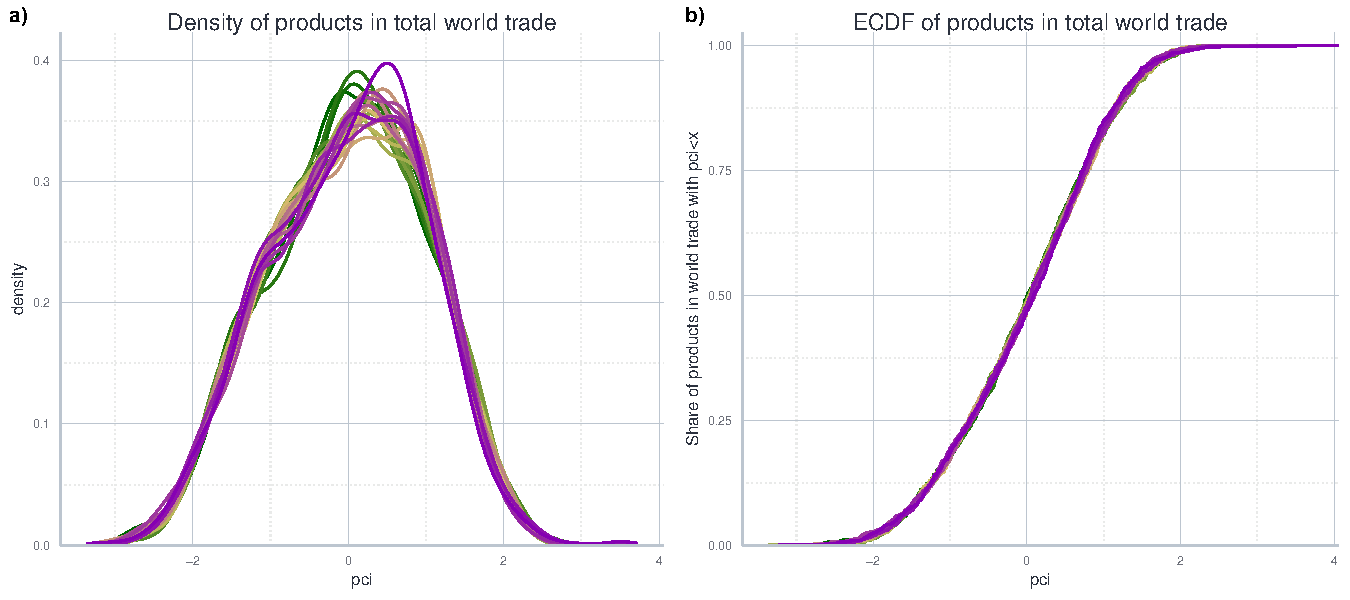
\includegraphics[width=\textwidth]{../output/fig_A1_dist-pci.pdf}
\caption{The distribution of products with regard to their complexity.
The different colors refer to the different years between 2000 and 2016.}
\label{fig:product-dist}
\end{figure}

\section{Complexity distribution of disaggregated export baskets}\label{ap:exp-densities}
Figure \ref{fig:exp-dens} shows a disaggregated version of figure 7a in the main text.
Here one sees both the within- and between group heterogeneity as described in section 3.2 of the main paper.

\begin{figure}[h]
\centering
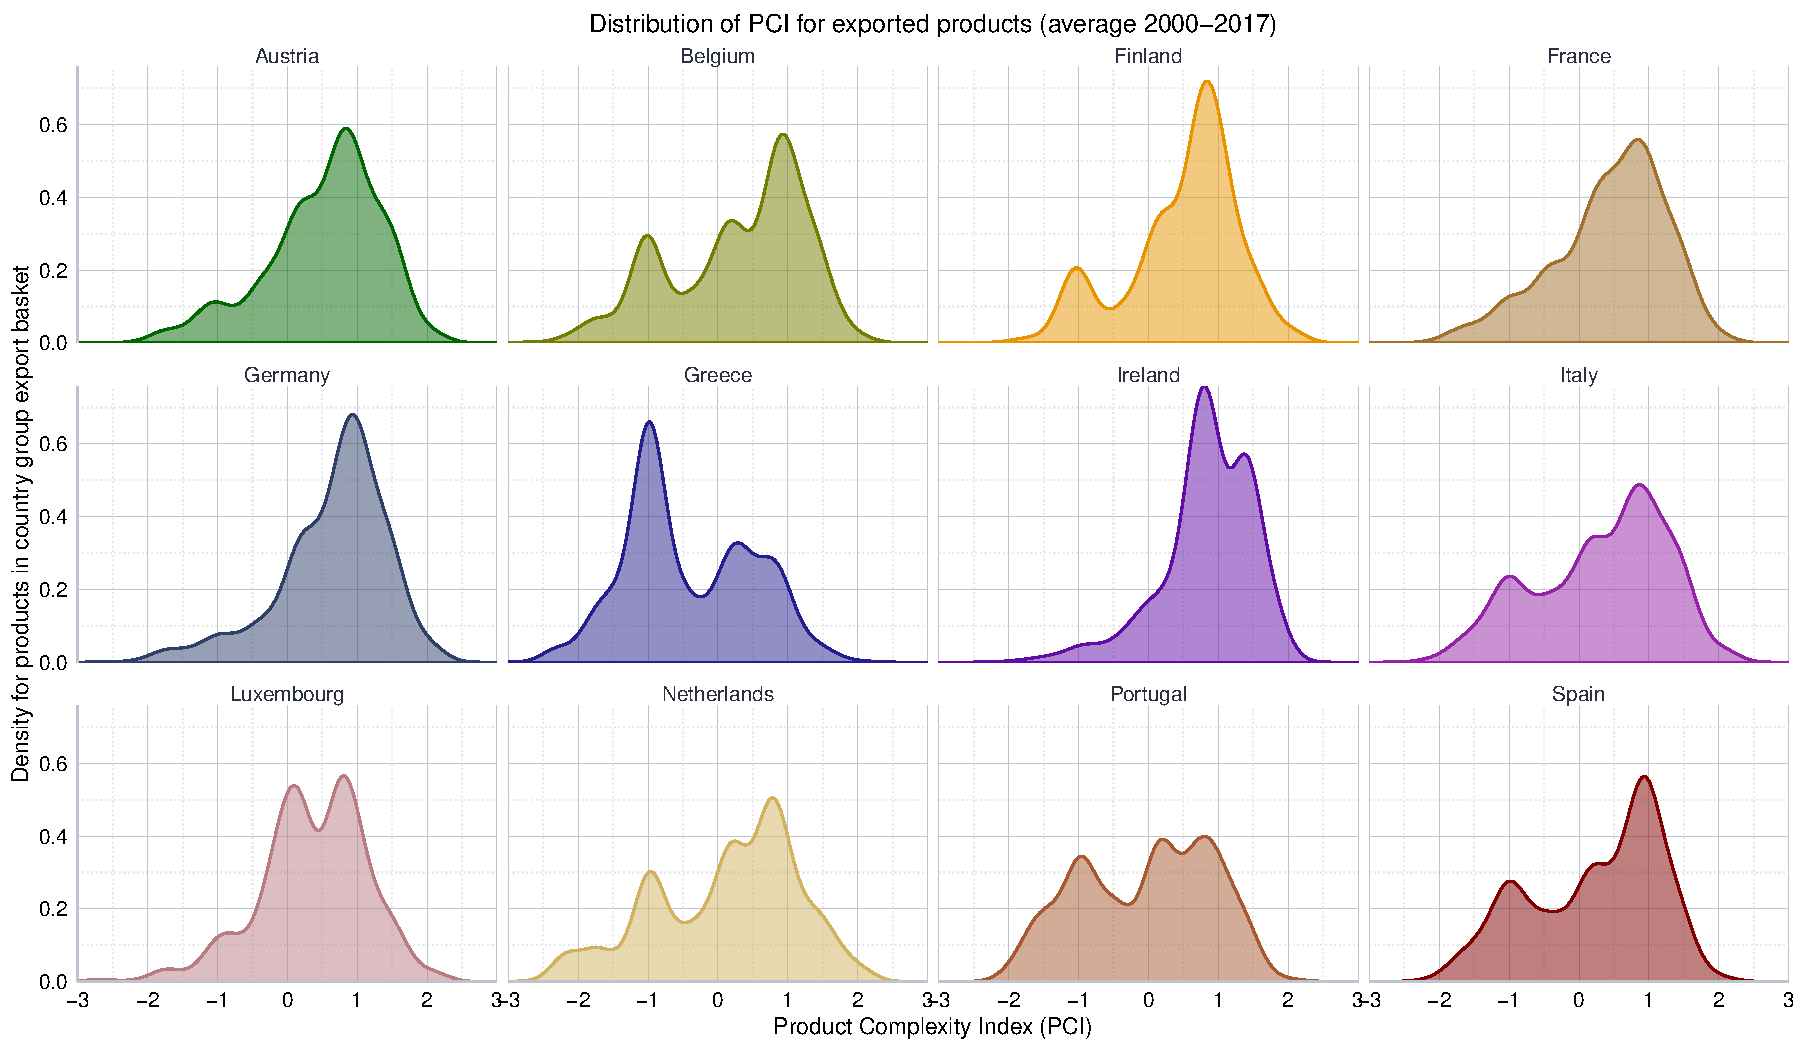
\includegraphics[width=\textwidth]{../output/fig_A2_exp_dists.pdf}
\caption{The PCI distribution of the average expert baskets from core and periphery countries between 2000 and 2017. A disaggregated version of figure 7a in the main text.}\label{fig:exp-dens}
\end{figure}

\clearpage
\printbibliography
\end{document}
